\documentclass[11pt]{article}
\usepackage[T1]{fontenc}
\usepackage[utf8]{inputenc}
\usepackage[a4paper,margin=1in]{geometry}
\usepackage{setspace}
\onehalfspacing
\setlength{\parskip}{0.5em}
\setlength{\parindent}{1.5em}
\usepackage{lineno}
\linenumbers
\usepackage{graphicx}
\usepackage{booktabs}
\usepackage{caption}
\usepackage{subcaption}
\usepackage{url}
\usepackage{amsmath}
\usepackage{float}
% Harvard / author–year citations
\usepackage[authoryear,round,semicolon,sort&compress]{natbib}
\title{Logistic models most frequently describe microbial growth curves across contexts}
\author{Yijia Yao\\Imperial College London}
\date{}
\begin{document}
% Auto wordcount (generated by Code/08_compile_report.sh).
% Fallback if the file doesn't exist yet (e.g. first compile):
\IfFileExists{wordcount.tex}{\input{wordcount.tex}}{\newcommand{\WordCount}{XXXX}}
% -----------------------
% Title page (separate)
% -----------------------
\begin{titlepage}
\centering
\vspace*{2cm}
{\LARGE \textbf{Logistic models most frequently describe microbial growth curves across contexts}\par}
\vspace{1.5cm}
{\large Yijia Yao\par}
\vspace{0.5cm}
{\large Imperial College London\par}
\vspace{1.5cm}
{\large Word count: \WordCount\par}
\vspace{1.5cm}
\begin{abstract}
Microbial growth curves are a familiar empirical pattern, but the most useful mathematical description is not always obvious because different models can fit similar trajectories for different reasons. Four candidate models for microbial abundance through time were compared: two phenomenological polynomials (quadratic and cubic) and two sigmoid growth models with interpretable structure (logistic and Gompertz). Each growth curve was defined as a unique Species--Temperature--Medium--Citation--Replicate combination. Models were fitted by least squares and the best-supported model within each curve was selected using AIC and BIC. Across 305 curves, 1178 of 1220 curve--model combinations were successfully fitted and 42 were skipped when parameters were not identifiable from the available time points. A best-supported model could be identified for 297 curves. The logistic model was selected most frequently (AIC: 124/297; BIC: 127/297), followed by the cubic polynomial (AIC: 81/297; BIC: 74/297) and the Gompertz model (68/297 under both criteria). Model discrimination was often weak: 143/297 curves had \(\Delta\)AIC\(_{\text{runner-up}}<2\). Logistic wins were particularly often marginal (61/124 weak wins), whereas cubic wins were more frequently decisive (33/81 with \(\Delta\)AIC\(_{\text{runner-up}}>10\)). Overall, a simple logistic form most often captured the dominant structure of microbial growth in this dataset, while the flexibility of cubic polynomials and the asymmetry of the Gompertz curve were advantageous for meaningful subsets of curves.
\end{abstract}
\end{titlepage}
% -----------------------
% Introduction
% -----------------------
\section*{Introduction}

Population growth is conceptually simple but methodologically rich because the same qualitative trajectory can be represented by multiple mathematical forms, each encoding different assumptions and degrees of mechanistic interpretation. Microbes grown in batch culture commonly show a lag phase, a period of approximately exponential increase, and a saturation phase as resources become limiting and inhibitory by-products accumulate \citep{Zwietering1990,MichaCorradini2011}. The resulting curve is typically sigmoidal, but different sigmoids imply different biological emphases. Logistic growth is a compact representation of density dependence and a carrying capacity, whereas the Gompertz curve allows asymmetric rise and saturation and has a long history of use in quantitative microbiology \citep{Zwietering1990,Buchanan1997}. In parallel, flexible phenomenological functions such as polynomials can describe curvature without attributing meaning to parameters; they often fit well but risk over-interpreting noise and may behave poorly outside the observed range \citep{MichaCorradini2011}.

This distinction matters because microbial growth is often used as a proxy for broader ecological performance. The speed with which a microbial population approaches saturation determines how quickly resources are exploited, how strongly density dependence emerges, and how sensitive system behaviour may be to environmental change. In practice, however, the available data do not always resolve these processes clearly. Some curves capture a full rise-and-plateau trajectory, whereas others include only the early phase of increase or a noisy partial series. Under those conditions, the model that appears best may partly reflect the informational content of the curve rather than a universally superior biological description.

When multiple models are plausible, model comparison is best framed as an explicit inferential problem rather than a purely visual choice. Information criteria provide a widely used framework for balancing goodness-of-fit against parameter count \citep{Akaike1974,Schwarz1978}. In ecological and evolutionary applications, this approach has become standard practice for comparing alternative hypotheses represented by alternative models \citep{JohnsonOmland2004,BurnhamAnderson2002}. However, nonlinear fitting can be fragile: convergence, starting values, bounds, and data resolution can all influence whether parameter estimation succeeds and whether models are distinguishable \citep{MotulskyChristopoulos2004,Bolker2013}. A model that wins often is therefore not necessarily one that is decisively better in every case.

The present analysis addresses the question of which mathematical model is most often best supported by microbial growth curves measured under diverse experimental contexts. Two polynomial benchmarks (quadratic and cubic) are compared with two widely used sigmoid growth models (logistic and Gompertz). Based on the biology of batch-culture growth, sigmoidal models were expected to perform well overall because they capture resource-limited saturation. At the same time, exploratory plots suggested that sparse curves and curves with weak dynamic range might favour polynomial descriptions because flexibility can compensate for limited information. The analysis therefore examines not only which model wins most often, but also how decisively those wins occur and how winner identity varies with curve properties.
% -----------------------
% Methods
% -----------------------
\section*{Methods}
\subsection*{Data}
The course-provided dataset \texttt{logistic\_growth\_data.csv} was used. It contains time-series measurements of microbial abundance or biomass (\texttt{PopBio}) through time (\texttt{Time}) across species/strains, temperatures, media, citations and experimental replicates. Time was recorded in hours. \texttt{PopBio} was recorded in heterogeneous units (e.g.\ optical density, CFU, counts, dry weight). Because measurement scale and error structure differ across units, model selection was performed \emph{within} each curve (models compared only on the same response scale), rather than by comparing residual magnitudes across curves \citep{BurnhamAnderson2002,JohnsonOmland2004}.
A single growth curve was defined by the unique combination of \texttt{Species}, \texttt{Temp}, \texttt{Medium}, \texttt{Citation}, and \texttt{Rep}. These fields were concatenated to construct a unique identifier (\texttt{curve\_id}) and a shorter numeric index (\texttt{curve\_num}) for plotting and tabulation. Within each curve, observations were ordered by time prior to fitting. Minor floating-point artefacts around Time \(=0\) were treated as zero for plotting only.
\subsection*{Candidate models}
For each curve, four candidate models describing \texttt{PopBio} as a function of time \(t\) were fitted:
\begin{enumerate}
\item \textbf{Quadratic polynomial} (phenomenological): \(y(t)=a t^2 + b t + c\).
\item \textbf{Cubic polynomial} (phenomenological): \(y(t)=a t^3 + b t^2 + c t + d\).
\item \textbf{Logistic growth} (sigmoid): \(y(t)=\dfrac{K}{1+\exp\{-r(t-t_0)\}}\), where \(K\) is an upper asymptote (carrying-capacity proxy), \(r\) is a growth-rate parameter, and \(t_0\) is an inflection-time parameter.
\item \textbf{Gompertz growth} (asymmetric sigmoid): \(y(t)=K\exp\{-\exp[-r(t-t_0)]\}\), where \(K\) is the upper asymptote, \(r\) controls the maximum growth rate near the inflection, and \(t_0\) is a timing parameter \citep{Zwietering1990,Buchanan1997}.
\end{enumerate}
Polynomial models provide flexible benchmarks but lack mechanistic interpretation and can extrapolate poorly outside the observed range \citep{MichaCorradini2011}. Logistic and Gompertz models are widely used primary growth models in microbiology and summarise multi-phase trajectories with interpretable parameters \citep{Zwietering1990,MichaCorradini2011}. In this report, logistic and Gompertz are treated as ``mechanistic-inspired'' rather than fully mechanistic: expected qualitative structure is captured and parameters remain interpretable, but explicit resource dynamics and physiological lag processes are abstracted away.
\subsection*{Model fitting}
All models were fitted by least squares using \texttt{scipy.optimize.curve\_fit}. For polynomial models, coefficients from \texttt{numpy.polyfit} were used as starting values. For sigmoid models, starting values were derived from each curve: \(K\) was initialised to the maximum observed \texttt{PopBio} (or slightly above), \(t_0\) to the median observed time, and \(r\) to a small positive value. To stabilise estimation across heterogeneous curves, bounds reflecting basic biological plausibility were imposed: \(K>0\), \(r>0\), and \(t_0\) constrained to fall within the observed time range. This bounded NLLS approach improves stability for heterogeneous datasets and reduces implausible solutions \citep{MotulskyChristopoulos2004,Bolker2013}.
Some curve--model combinations were \textbf{skipped} when parameters were not identifiable from the available time points. Specifically, if a curve had fewer than \(k+1\) unique time values (where \(k\) is the number of free parameters in the model), the fit was not attempted. Skipped fits were treated as data-resolution limitations rather than numerical failures \citep{Bolker2013}.
\subsection*{Model selection and evidence strength}
For each fitted curve--model combination, residual sum of squares (RSS) was calculated and used to compute AIC and BIC under a Gaussian error model with constant variance. With \(n\) observations and \(k\) fitted parameters, the following standard least-squares forms were used \citep{Akaike1974,Schwarz1978}:
\[
\mathrm{AIC} = n\ln\left(\frac{\mathrm{RSS}}{n}\right) + 2k,
\qquad
\mathrm{BIC} = n\ln\left(\frac{\mathrm{RSS}}{n}\right) + k\ln(n).
\]
Models were compared only within the same curve. The winning model for each curve was the one with minimum AIC (or BIC). To quantify how decisively the winner was preferred, the AIC gap between the best and second-best model within each curve was computed as \(\Delta\)AIC\(_{\text{runner-up}}\), and evidence was summarised using conventional thresholds (\(<2\), 2--7, 7--10, \(>10\)) \citep{BurnhamAnderson2002}. Representative fitted curves were inspected visually to ensure that low information criteria corresponded to sensible fitted shapes rather than pathological parameterisations.
\subsection*{Computing tools}
All analysis steps were implemented in Python and executed from a single entry point (\texttt{run\_MiniProject.py}), which runs data preparation, exploratory plotting, model fitting, model comparison, and summary steps sequentially. Data handling used \texttt{pandas}; numerical operations used \texttt{numpy}; plotting used \texttt{matplotlib}; and model fitting used \texttt{scipy}. Git was used for version control. The report was written in \LaTeX{} and compiled via a shell script to make document generation reproducible.
% -----------------------
% Results
% -----------------------
\section*{Results}
\subsection*{Data overview and fitting coverage}
A total of 305 unique growth curves were identified, and four models were attempted per curve (1220 curve--model combinations). Model fitting succeeded for 1178 combinations, and 42 combinations were skipped due to insufficient unique time points for parameter identifiability. A best-supported model (AIC/BIC computable and comparable) could be identified for 297 curves. Seven curves contained at least one non-positive \texttt{PopBio} value, consistent with measurement noise or background-correction artefacts, which restricts the use of naive log transformations without additional handling.
These curves varied substantially in shape, scale, and resolution. Some showed clear sigmoidal trajectories with an evident rise and plateau, whereas others were shorter, noisier, or only partially captured the underlying process. This variation in information content is important because it constrains how strongly alternative models can be distinguished.
\subsection*{Overall model performance}
Under AIC, the logistic model was selected most frequently (124/297 curves; 41.8\%), followed by the cubic polynomial (81/297; 27.3\%), the Gompertz model (68/297; 22.9\%), and the quadratic polynomial (24/297; 8.1\%). The pattern was similar under BIC, which slightly increased support for the logistic model (127/297; 42.8\%) and reduced support for the cubic polynomial (74/297; 24.9\%) (Table~\ref{tab:win_summary}; Figure~\ref{fig:wins_aic}). Overall, the ranking logistic \(>\) cubic \(>\) Gompertz \(>\) quadratic was consistent across both criteria.

The overall pattern in Figure~\ref{fig:wins_aic} is clear, with logistic growth emerging as the modal winner across the dataset, but not to the exclusion of all alternatives. Cubic and Gompertz models together account for a substantial fraction of winning fits, indicating that while saturation is a common feature of microbial growth trajectories, many curves either depart from a simple symmetric sigmoid or do not contain enough information for a simple sigmoid to be clearly preferred. Figure~\ref{fig:wins_by_unit} further suggests that winner identity is not fully invariant across response units. This is relevant because different measurement types may emphasise different aspects of growth dynamics and may differ in observational noise, even when the underlying biological process is similar.
\begin{table}[H]
\centering
\caption{Model win counts under AIC and BIC (n=297 curves with an identifiable winner).}
\label{tab:win_summary}
\begin{tabular}{lrrrr}
\toprule
Model & AIC wins & BIC wins & Total (AIC) & Total (BIC) \\
\midrule
Logistic  & 124 & 127 & 297 & 297 \\
Cubic     & 81  & 74  & 297 & 297 \\
Gompertz  & 68  & 68  & 297 & 297 \\
Quadratic & 24  & 28  & 297 & 297 \\
\bottomrule
\end{tabular}
\end{table}
\begin{figure}[H]
\centering
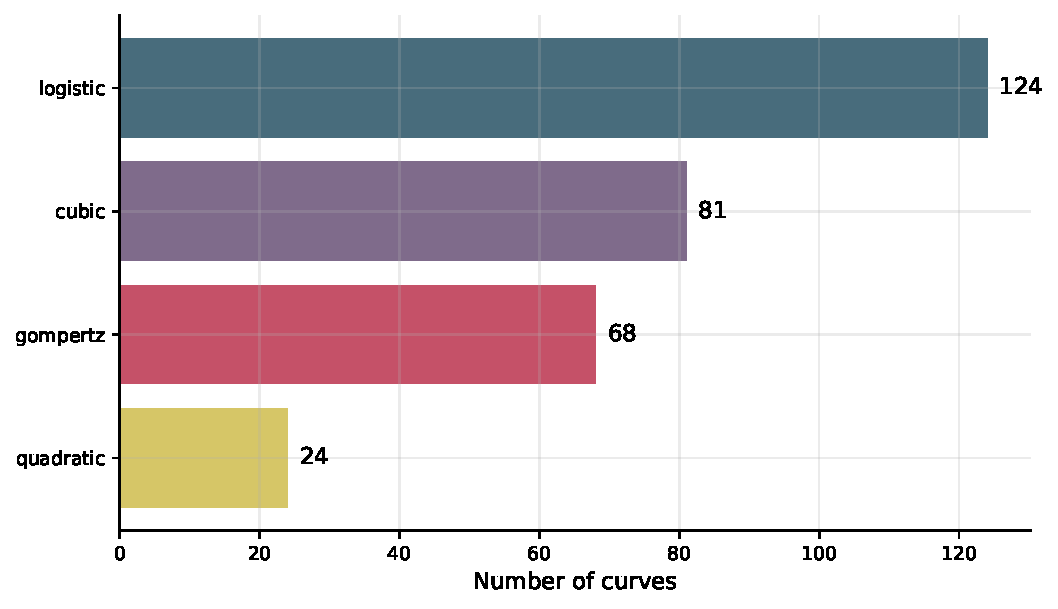
\includegraphics[width=0.82\textwidth]{../Results/Figures/model_wins_aic.pdf}
\caption{\textbf{Overall model winners across growth curves under AIC.} Bars show how often each model achieved the lowest AIC within a growth curve (n=297 curves with an identifiable winner). Logistic growth was selected most often, with cubic polynomials and the Gompertz model providing better support for substantial subsets of curves.}
\label{fig:wins_aic}
\end{figure}
\begin{figure}[H]
\centering
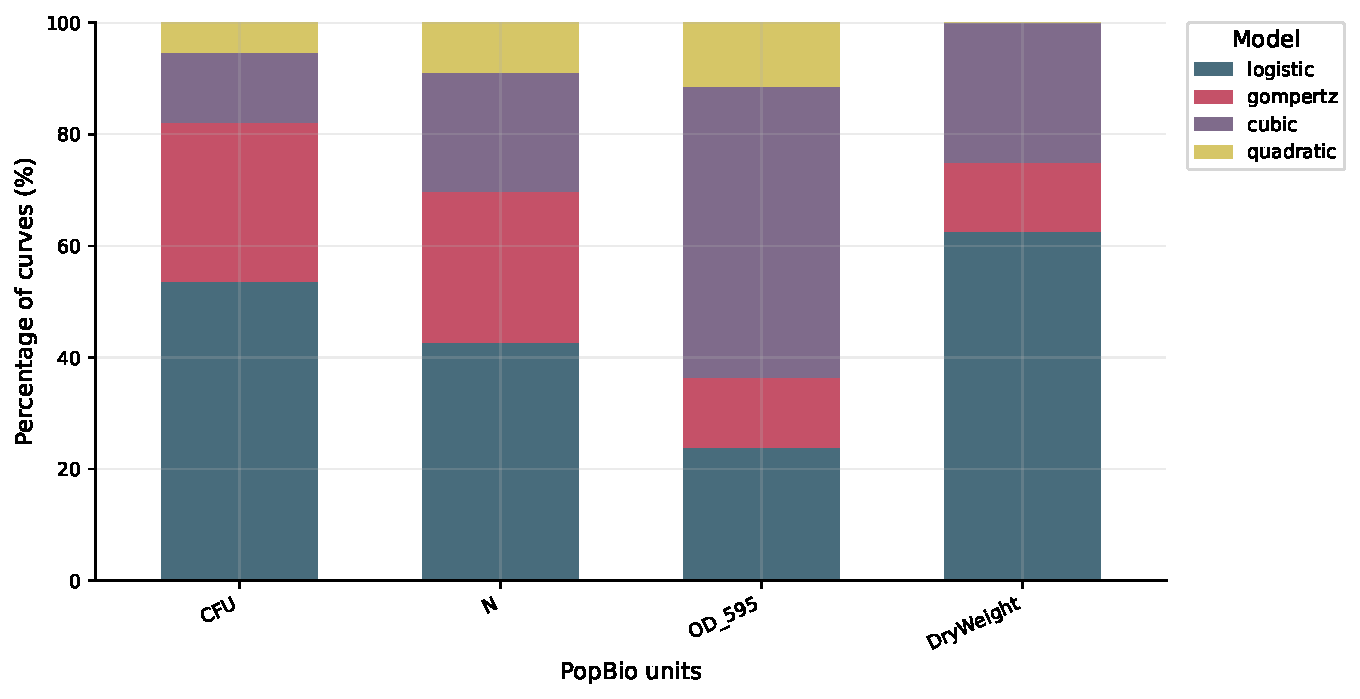
\includegraphics[width=0.95\textwidth]{../Results/Figures/model_wins_by_unit_aic.pdf}
\caption{\textbf{AIC-winning models stratified by response units.} Winners are shown separately for different \texttt{PopBio} measurement scales. The relative frequency of polynomial vs.\ sigmoid winners varies among units, consistent with heterogeneous curve shapes and noise structures across experimental contexts.}
\label{fig:wins_by_unit}
\end{figure}
\subsection*{Evidence strength of model selection}
Win counts alone can obscure whether the winning model is clearly preferred or only marginally better than its closest competitor. Across 297 curves, discrimination was frequently weak: 143 curves (48.1\%) had \(\Delta\)AIC\(_{\text{runner-up}}<2\), indicating that multiple models fit nearly equally well. A further 63 curves (21.2\%) showed moderate support (2--7), 31 curves (10.4\%) strong support (7--10), and 60 curves (20.2\%) very strong support (\(>10\)) for the winner \citep{BurnhamAnderson2002}.
Evidence strength differed among winners. Logistic wins were often marginal: 61/124 (49.2\%) of logistic-winning curves had \(\Delta\)AIC\(_{\text{runner-up}}<2\). Gompertz wins were similarly often weak (35/68, 51.5\% weak) and only rarely very strong (4/68, 5.9\%). In contrast, cubic wins were more frequently decisive: 33/81 (40.7\%) of cubic-winning curves had \(\Delta\)AIC\(_{\text{runner-up}}>10\). This pattern suggests that many curves do not contain sufficient information to confidently discriminate among similar sigmoids, whereas a subset contains departures from simple sigmoid structure that are captured much better by more flexible functions.
\begin{figure}[H]
\centering
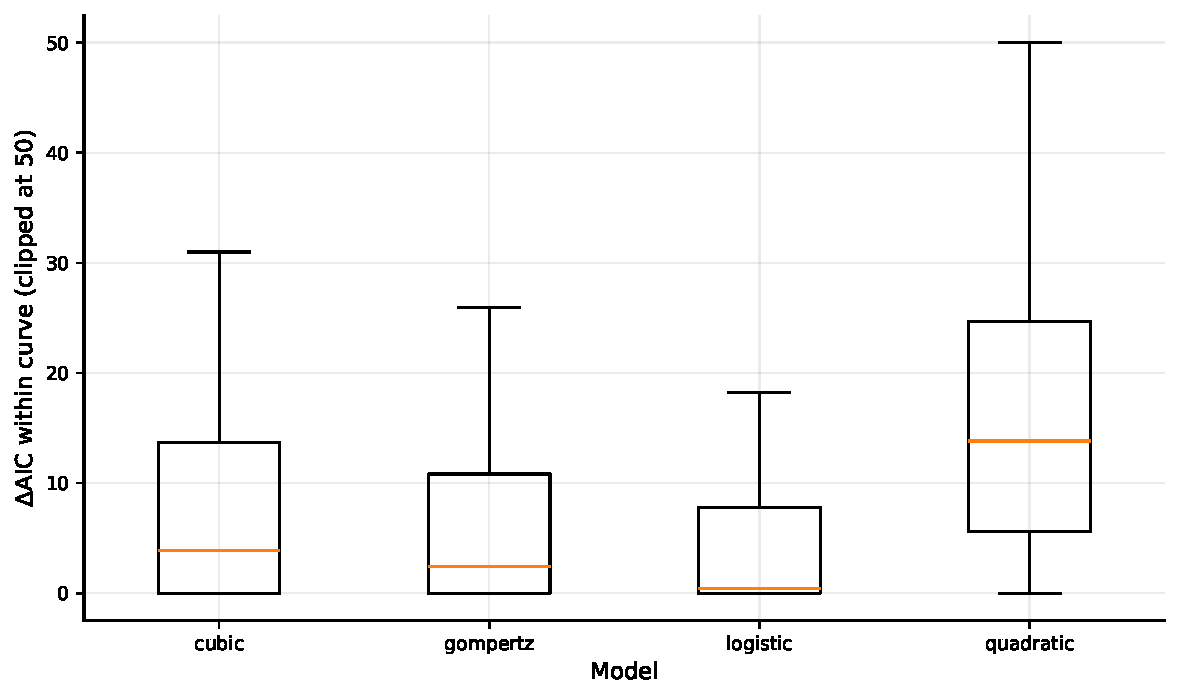
\includegraphics[width=0.9\textwidth]{../Results/Figures/deltaAIC_distribution.pdf}
\caption{\textbf{Within-curve \(\Delta\)AIC distributions across models.} For each growth curve, \(\Delta\)AIC is computed as AIC minus the minimum AIC among the four candidate models for that curve. Values close to 0 indicate near-best fits, whereas larger values indicate poorer support within that curve.}
\label{fig:deltaAIC_distribution}
\end{figure}
\begin{figure}[H]
\centering
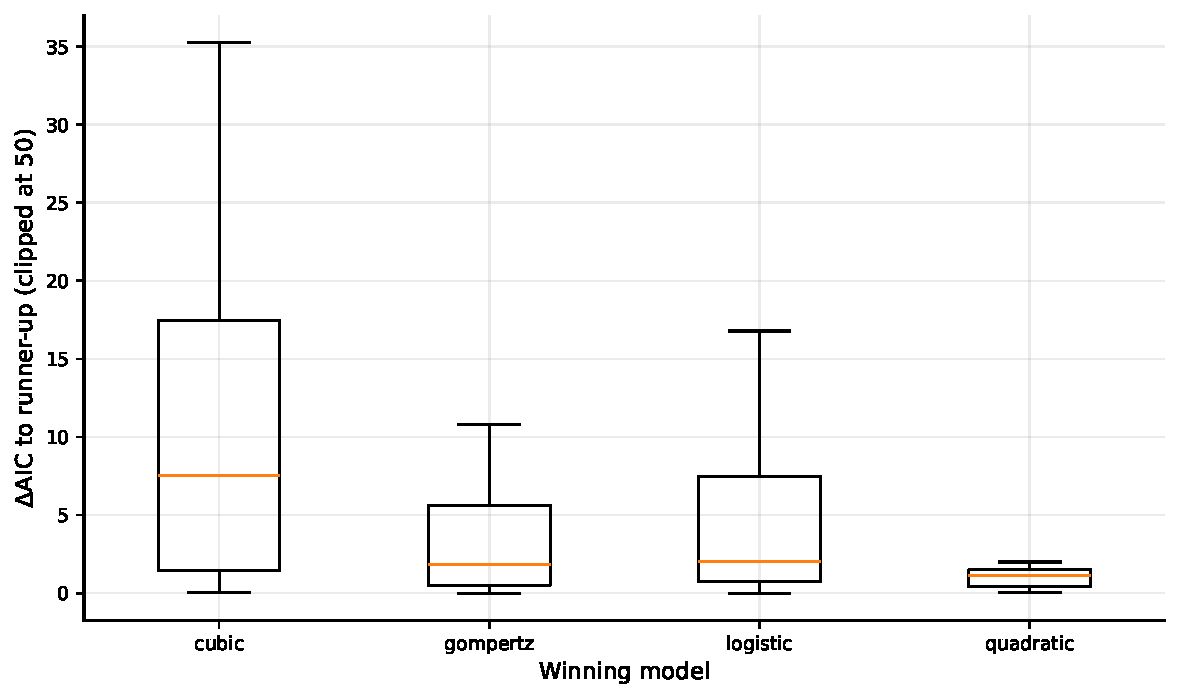
\includegraphics[width=0.9\textwidth]{../Results/Figures/deltaAIC_winner_strength.pdf}
\caption{\textbf{Evidence strength of AIC winners.} For each curve, the AIC gap between the best and second-best model (\(\Delta\)AIC\(_{\text{runner-up}}\)) summarises how decisively the winner is preferred. Small gaps (\(<2\)) indicate weak discrimination among models; large gaps (\(>10\)) indicate strong support for the winner.}
\label{fig:deltaAIC_strength}
\end{figure}
From an interpretive perspective, this result is crucial because it prevents the overall winner counts from being overstated. A model that wins frequently but only by very small AIC differences should not be treated as universally superior. Instead, the evidence-strength results suggest that many curves are informative about broad saturation behaviour without being sufficiently resolved to identify the exact functional form of that saturation.
\subsection*{Model wins in relation to sampling density and curve scale}
Model winners were not evenly distributed across curve informativeness. The number of observations per curve influenced which model was selected (Table~\ref{tab:winner_npoints}; Figure~\ref{fig:winner_npoints}). For sparsely sampled curves (\(\leq 10\) points), the logistic model won most often, consistent with its ability to summarise overall sigmoid structure with relatively few parameters. As sampling density increased (20--30 points), cubic wins became relatively more common, consistent with better-resolved curvature providing the information needed to justify additional flexibility.
\begin{table}[H]
\centering
\caption{AIC winners stratified by sampling density (number of observations per curve).}
\label{tab:winner_npoints}
\begin{tabular}{lrrrr}
\toprule
$n$ points bin & Cubic & Gompertz & Logistic & Quadratic \\
\midrule
$\leq 10$      & 29 & 25 & 62 & 4 \\
10--15         & 18 & 25 & 38 & 9 \\
15--20         & 12 & 11 & 12 & 4 \\
20--30         & 21 & 3  & 10 & 7 \\
$\geq 30$      & 1  & 3  & 1  & 0 \\
\bottomrule
\end{tabular}
\end{table}
Winner patterns also depended on within-curve variation (dynamic range; Table~\ref{tab:winner_dyn}; Figure~\ref{fig:winner_dyn}). In the lowest dynamic-range quartile, cubic polynomials dominated, whereas logistic wins increased with dynamic range. When a curve does not span a large range of \texttt{PopBio} values, both rapid growth and saturation may be poorly resolved; in that setting, polynomials can fit shallow curvature without requiring a well-identified plateau. Conversely, when dynamic range is large, saturation becomes more detectable and logistic structure is more strongly supported. Gompertz winners were concentrated in the highest dynamic-range quartile, consistent with asymmetry becoming detectable only when curves span sufficient range and are sampled densely enough.
\begin{table}[H]
\centering
\caption{AIC winners stratified by within-curve \texttt{PopBio} dynamic-range quartiles.}
\label{tab:winner_dyn}
\begin{tabular}{lrrrr}
\toprule
Dynamic-range quartile & Cubic & Gompertz & Logistic & Quadratic \\
\midrule
Q1 (lowest)  & 39 & 5  & 16 & 15 \\
Q2           & 22 & 26 & 26 & 0 \\
Q3           & 16 & 13 & 44 & 1 \\
Q4 (highest) & 4  & 24 & 38 & 8 \\
\bottomrule
\end{tabular}
\end{table}
\begin{figure}[H]
\centering
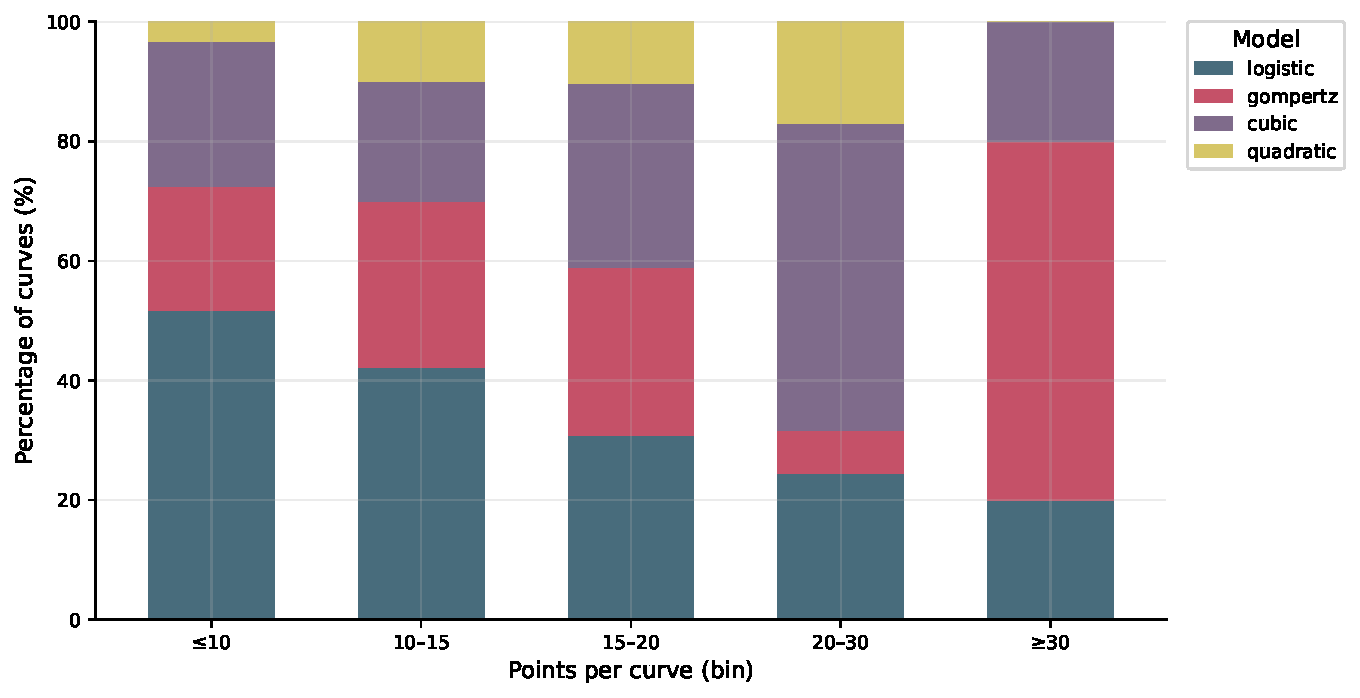
\includegraphics[width=0.95\textwidth]{../Results/Figures/winner_by_npoints_stacked.pdf}
\caption{\textbf{AIC-winning model composition stratified by sampling density.} Bars show the percentage of curves (within each bin of number of observations) for which each model is the AIC winner. Better-sampled curves show a higher fraction of polynomial wins, consistent with additional curvature becoming detectable.}
\label{fig:winner_npoints}
\end{figure}
\begin{figure}[H]
\centering
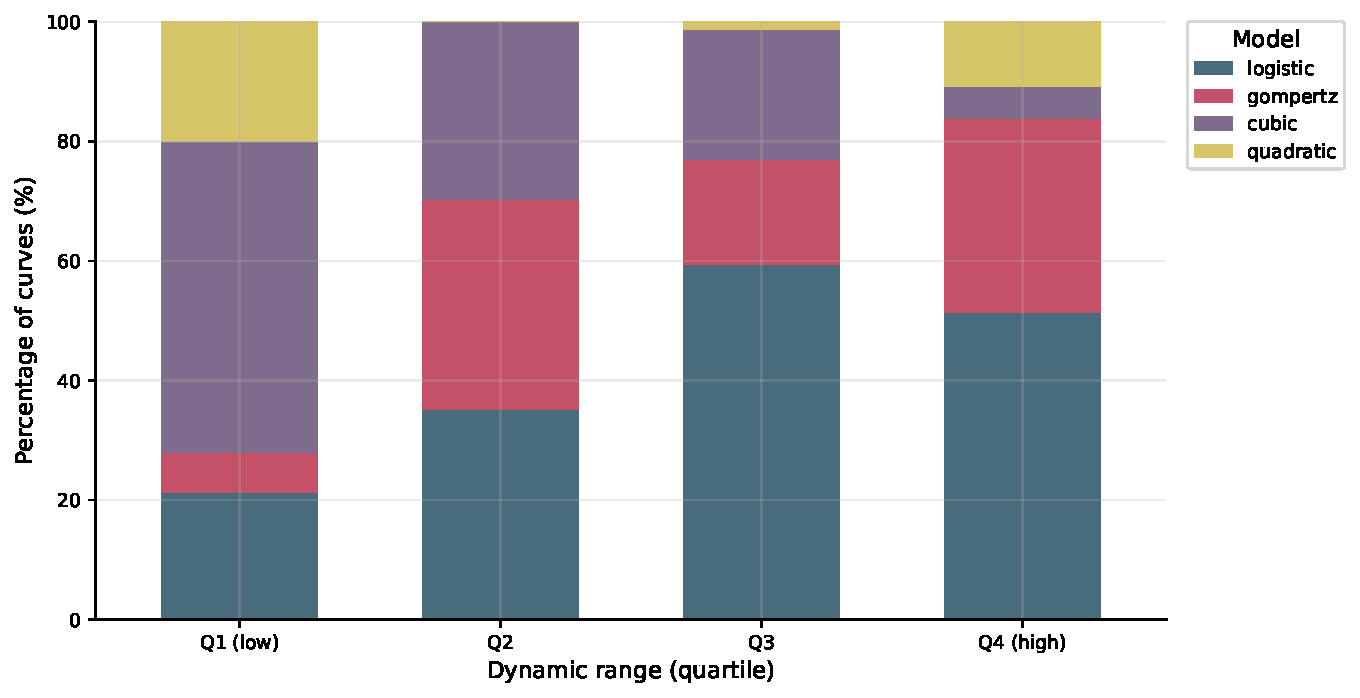
\includegraphics[width=0.95\textwidth]{../Results/Figures/winner_by_dynamicrange_stacked.pdf}
\caption{\textbf{AIC-winning model composition stratified by dynamic range.} Bars show the percentage of curves (within each dynamic-range quartile) for which each model is the AIC winner. Logistic wins increase with dynamic range, whereas cubic wins dominate low dynamic-range curves, consistent with weakly informative trajectories where sigmoid structure is hard to distinguish.}
\label{fig:winner_dyn}
\end{figure}
Taken together, these patterns show that model support depended not only on model form, but also on the informational content of the data. In curves with low dynamic range, the distinction between true saturation and shallow curvature is inherently difficult to resolve, so flexible polynomial models can compete successfully even when a sigmoidal biological process may underlie the data. In contrast, when curves span a broader range and include a more complete trajectory, carrying-capacity-like behaviour becomes more visible and sigmoidal models gain support. The shift from polynomial to sigmoidal winners across data-rich curves therefore reflects not only statistical fit, but also the increasing visibility of ecologically meaningful structure.
% -----------------------
% Discussion
% -----------------------
\section*{Discussion}
Across diverse microbial growth curves, the logistic model was most frequently best supported under both AIC and BIC. Many trajectories exhibit a clear approach to a plateau, and logistic growth summarises that structure parsimoniously. BIC in particular rewards models that capture dominant patterns without unnecessary flexibility \citep{Schwarz1978,Raftery1995}. The Gompertz model, although selected less often overall, still won for nearly a quarter of curves, suggesting that asymmetric rise versus saturation is common but not universal in this dataset, consistent with previous comparisons of primary growth models \citep{Zwietering1990,Buchanan1997}.

A key insight from the \(\Delta\)AIC analysis is that ``winning'' often reflects marginal differences rather than decisive evidence, as almost half of curves had \(\Delta\)AIC\(_{\text{runner-up}}<2\). In such cases, multiple model classes can reproduce the observed data equally well, either because curves are sparsely sampled, because measurement noise dominates subtle shape differences, or because curves do not span enough dynamic range to clearly reveal both rapid growth and saturation. When discrimination is weak, model choice is often better guided by interpretability and intended use than by small information-criterion differences \citep{BurnhamAnderson2002,JohnsonOmland2004}. This is particularly relevant for logistic winners: nearly half were weak wins, implying that logistic growth is frequently a reasonable default summary but not uniquely supported by the data.

The stratified analyses help explain why support shifted across the dataset. Logistic wins increased with dynamic range, consistent with density-dependent slowing and saturation being most detectable when curves span a large biological signal. Gompertz winners were concentrated in the highest dynamic-range quartile, suggesting that asymmetry becomes easier to detect when both the rise phase and the approach to the asymptote are well resolved. By contrast, cubic wins dominated low dynamic-range curves and became relatively more common in better-sampled bins. This suggests that flexible polynomials are not simply overfitting at random; rather, they can either absorb weakly informative shallow curvature or accommodate genuine departures from idealised sigmoid structure when sufficient detail is present.

These results highlight a central ecological and statistical trade-off. Logistic and Gompertz models are attractive because they compress growth into interpretable parameters that can, in principle, be compared across taxa or environments. However, flexible phenomenological models can outperform them when trajectories contain late-stage deviations, mild downturns, or irregularities not represented by simple sigmoids. This does not mean that polynomial models necessarily provide better ecological explanation; rather, they may provide a better empirical description of imperfect or more complex data. A stronger interpretation therefore lies not in declaring one model universally superior, but in recognising that model performance depends on the balance between interpretability and flexibility.

This trade-off matters beyond this dataset. In predictive microbiology, growth models are often used to estimate when microbial populations approach thresholds relevant to spoilage or unsafe abundance. In ecological contexts, similar models are used to compare how rapidly populations exploit resources or how strongly growth slows under environmental constraint. If model discrimination is weak, downstream interpretation of fitted parameters must remain cautious: a parameter may look biologically meaningful simply because it belongs to an interpretable model, even when an alternative formulation fits almost as well. The present results therefore argue for interpreting microbial growth parameters in light of evidence strength, not winner identity alone.

Several limitations should also be acknowledged. First, \texttt{PopBio} was measured in heterogeneous units, implying different error structures and potential heteroskedasticity; inference was therefore restricted to within-curve comparisons. Second, log-scale approaches that can stabilise variance were not universally applicable because seven curves contained non-positive \texttt{PopBio} values. Third, skipped fits reflected genuine data-resolution constraints and showed that model complexity must match curve informativeness. Finally, logistic and Gompertz models compress multi-phase microbial growth into simple sigmoids; models that explicitly represent lag-phase dynamics, such as Baranyi-type approaches, could provide a useful next step if the aim were physiological inference about lag rather than comparative description \citep{BaranyiRoberts1994,Buchanan1997}.
The results also suggest that some apparent model differences may reflect missing biological structure. For example, cubic wins may partly arise because some trajectories contain late-stage downturns, shifts in curvature, or lag-related departures that simple logistic and Gompertz forms do not represent explicitly. In such cases, a polynomial can provide a better empirical description without necessarily providing a better ecological explanation. This strengthens the case for expanding the candidate model set in future analyses to include models that preserve biological interpretability while accommodating more realistic microbial dynamics.
Several extensions follow naturally from these results. Candidate model sets could be expanded to include lag-explicit and decline-phase models, especially for curves where cubic fits were strongly preferred. In particular, logistic growth could be extended by adding an explicit lag component, as in Baranyi-type formulations, which may better capture temperature-dependent acclimation and delayed onset of growth \citep{BaranyiRoberts1994,Buchanan1997}. Predictive performance could also be assessed using cross-validation rather than relying solely on in-sample information criteria, allowing the distinction between descriptive fit and predictive utility to be tested more directly. In addition, variation among taxa, temperatures, media, or response units could be analysed more explicitly using hierarchical or mixed-effects frameworks, allowing the conditions under which different models succeed to be quantified directly. Finally, residual structure could be examined more formally to determine whether some apparent polynomial advantages arise from variance structure rather than from genuinely different biological shape.

Overall, the central conclusion is robust: across this dataset, logistic growth most often captured the dominant empirical structure of microbial growth curves, but model discrimination was frequently weak and subsets of curves showed strong support for alternative shapes. The most informative practice is therefore not only to report which model wins most often, but also to report how decisive those wins are and what level of biological interpretation each model permits.
% -----------------------
% References
% -----------------------
\setlength{\bibhang}{0.3in}
\setlength{\bibsep}{0.1in}
\newpage
\bibliographystyle{apalike}
\bibliography{references}
\end{document}